\documentclass[12pt]{article}
\usepackage{graphicx}
\usepackage{caption}
\usepackage{amsmath}
\usepackage{amssymb}
\usepackage{booktabs}
\usepackage{geometry}
\usepackage{float}
\usepackage{booktabs}
\usepackage{longtable}
\usepackage{setspace} % for spacing control
\usepackage{indentfirst}
\usepackage{titlesec}
\usepackage[most]{tcolorbox}

\newtcbtheorem{Summary}{\bfseries Summary}{enhanced,drop shadow={black!50!white},
  coltitle=black,
  top=0.3in,
  attach boxed title to top left=
  {xshift=1.5em,yshift=-\tcboxedtitleheight/2},
  boxed title style={size=small,colback=pink}
}{summary}


\newtcolorbox{summary}[2][]{%
  enhanced,
  drop shadow={black!50!white},
  coltitle=black,
  top=0.3in,
  attach boxed title to top left={xshift=1.5em,yshift=-\tcboxedtitleheight/2},
  boxed title style={size=small,colback=pink},
  title={\bfseries #2}, % manual title here
  #1
}

\setstretch{1.0}       % single line spacing (default)
\setlength{\parskip}{0pt}   % no space between paragraphs
\setlength{\parindent}{0em} % set indentation amount

\geometry{margin=1in}
\setlength{\parskip}{0em}
\setlength{\parindent}{0pt}

\title{Self-Evaluation Report \\ \large Computational Plasticity (SoSe25)}
\author{Bagus Alifah Hasyim \\ 108023246468}
\date{}

\begin{document}
\maketitle

\section*{Phenomenology of Plasticity}

\section{Difference between elastic and plastic strain}
\hspace{2em}To understand the difference between elastic and plastic strain, a simple visualization of a simple stress-strain
curve can be shown as following figure. 
\begin{figure}[H]
    \centering
    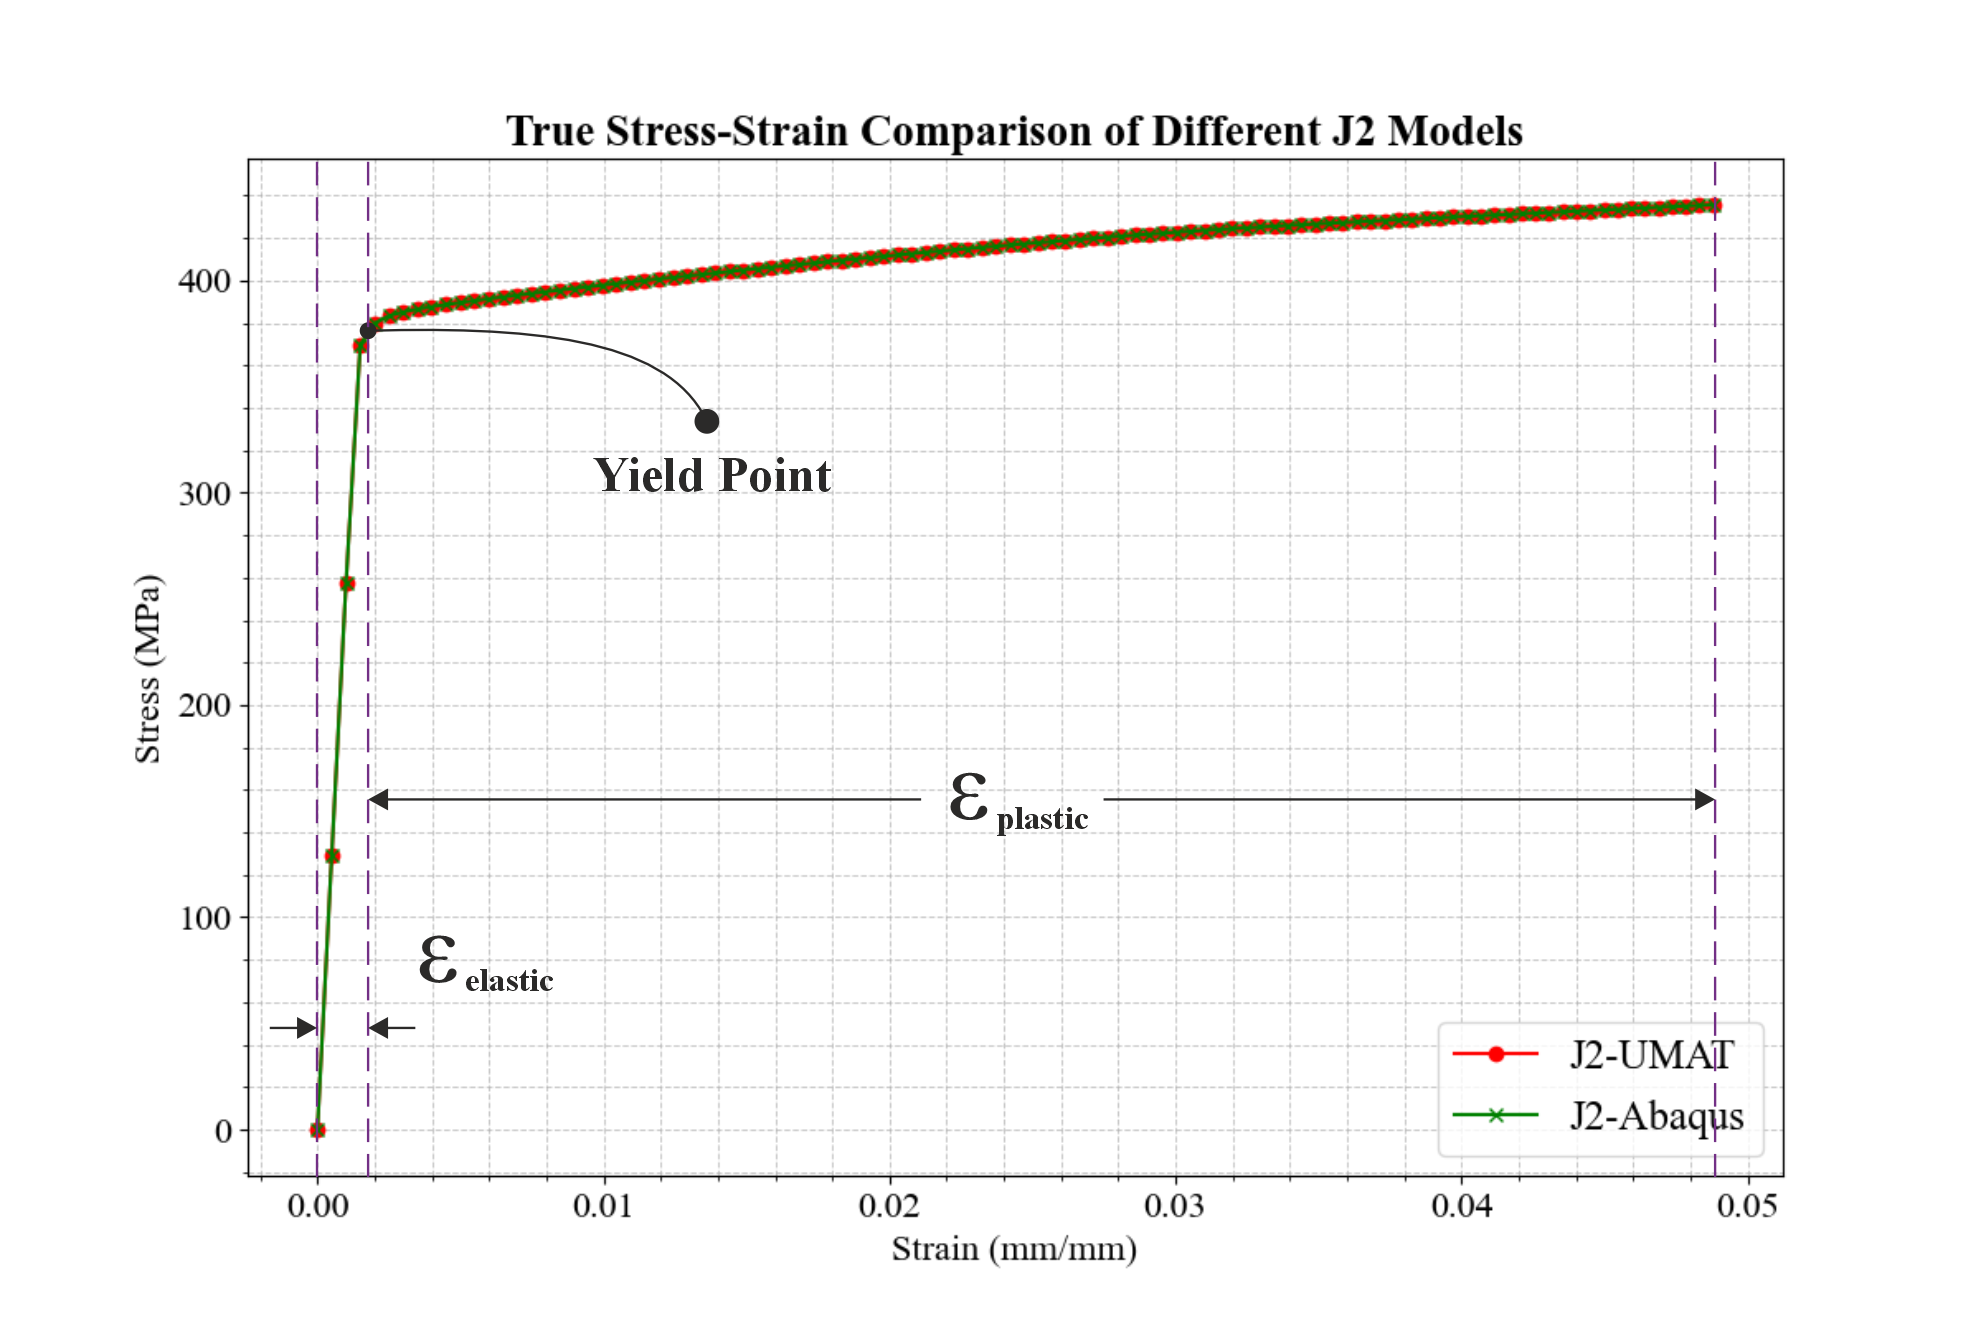
\includegraphics[width=0.8\textwidth]{images/StressStrain.png}
    \caption{A simple stress-strain curve that shows the elastic and plastic strain region. The yield point is the transition point from 
    elastic to plastic region.}
    \label{fig:stress_strain_curve}
\end{figure}

\hspace{2em}
As the material loaded with some external force, it will start to deform elastically. Here, the relation
between the stress (Y-Axis) and strain (X-Axis) shown a linear behavior until it reach a point where the materials start to yield.
The distance between the 0 point and yield point in X direction is called \textbf{elastic strain}. In a microscopic sense, the atoms are
displaced slightly in the direction of loading, which here there will be no displacement in between the atom. The bond, such 
as grain boundaries and atomic orientation will remain unchanged in this phase. Meaning that this is a reversible process. As the material exceeds the yield point, the deformation behavior will change. The material will not deformed elastically anymore, 
but rather plastically, in a microscopic sense that there will be some dislocation or a significant move in between the atomic bond
inside the material. Hence, this stage generates a non-linear stress-strain relationship, by means that the material will experience
a permanent deformation, in other words a non-reversible process. Hence, this phenomenon is called \textbf{plastic strain}. 

\section{Microscopic origin of plastic deformation}
\hspace{2em}
To elaborate more detail about the microscopic phenomenology on plastic deformation, explaining the key idea on microscopic 
scale of material should be done beside understanding it on a stress-strain curve. In general for a single crystal deformation, 
the loading will create a shear strain with respect to the crystal slip plane over another. This induced shear stress will cause
then will create a relative lateral movement from both parallel planes~\cite{taylor1934plastic}. 

\hspace{2em}
Based on theories of the equilibrium of crystal lattices, an atom should place itself in a minimum potential energy position
with respect to its neighbors. Whenever the atom moves, it will create heat internally. These minimum potential energy
will create "potential barriers", that restrict the atom to dislocate in between planes. As the dislocation exceed the
potential barrier, the atoms neighborhoods will rearrange themselves by a continuous process so that it will create a 
new equilibrium energy~\cite{taylor1934plastic}. This will create a new energy barriers, and the atoms position will not go back to
its origin since it has a new potential barrier. To introduce the same behavior again regarding the atom dislocation, 
one should apply condition where it will dislocate the atoms until it reach the updated minimum potential barriers.

\hspace{2em}From this idea, the plastic deformation can be explained as the dislocation movement
in between the crystal plane. The "permanent change" of the crystal lattice, which hence describe by the 
change of the potential barrier, highlight the plastic deformation. Once the barriers are exceeded, then
the plastic deformation state will occurs. 
\section*{Continuum Plasticity}
\section{Equivalent stress and yield function}
\hspace{2em}
The idea of equivalent stress is that there are needs to describe stress state in a unified or a scalar quantity
that can be compared to other quantities such as yield strength. Because as the material loaded by some external forces or traction,
it can introduce stress generation that has variation in terms of direction. To represent the stress component in each
direction, equivalent stress is used to model the stress state in the material. Because from the analysis, the stress result
can be only compared with material data that is obtained through an uniaxial tensile test. Here, the data only describe
the material flow in one direction of loading. To describe the stress in more detail, one can write the stress decomposition:
\begin{equation}
\boldsymbol{\sigma} = \boldsymbol{\sigma}_{hydro} + \boldsymbol{\sigma}_{dev}
\end{equation}

Where the hydrostatic stress is the stress component that cause a volumetric change of the material and 
the deviatoric stress component will cause shape change, which here for instance a distortion in the material. The
hydrostatic stress can be defined as follow:
\begin{equation}
\boldsymbol{\sigma}_{hydro} = \frac{1}{3} \text{tr}(\boldsymbol{\sigma}) \boldsymbol{I} = \frac{1}{3} \left( \sigma_{xx} + \sigma_{yy} + \sigma_{zz} \right) \boldsymbol{I}
\end{equation}

Then we are interested in the deviatoric stress component, which can be defined as:
\begin{equation}
\boldsymbol{\sigma}_{dev} = \boldsymbol{\sigma} - \boldsymbol{\sigma}_{hydro}
\end{equation}

By inserting the full stress component, we can write the deviatoric stress component as a full stress component in a matrix component
In this sense:
\begin{equation}
\boldsymbol{\sigma}_{dev} =
    \begin{bmatrix}
    \sigma_{xx} - \frac{1}{3}\text{tr}(\boldsymbol{\sigma}) & \sigma_{xy} & \sigma_{xz} \\
    \sigma_{yx} & \sigma_{yy} - \frac{1}{3}\text{tr}(\boldsymbol{\sigma}) & \sigma_{yz} \\
    \sigma_{zx} & \sigma_{zy} & \sigma_{zz} - \frac{1}{3}\text{tr}(\boldsymbol{\sigma})
    \label{eq:deviatoric_stress}
    \end{bmatrix}
    = s_{ij}
\end{equation}

Introducing the second deviatoric stress invariant $J_2$, which is a scalar quantity that can be used to describe the equivalent stress.
Hence, it can be denoted as follows:
\begin{equation}
J_2 = \frac{1}{2}s_{ij}s_{ij} = \frac{1}{2}[\text{tr}(s)^2-\text{tr}(s^2)]
\end{equation}

\begin{equation}
    J_2 = \frac{1}{2} \left((s_{11}^2 + s_{22}^2 + s_{33}^2 + 2(s_{12}^2 + s_{13}^2 + s_{23}^2)) \right)
\end{equation}

To obtain the $J_2$ in a stress component that describe in equation~\ref{eq:deviatoric_stress}, 
the $s_{ij}$ stress component can be inserted into the $J_2$ equation, hence it's written as follows:
\begin{equation}
    J_2 = \frac{1}{6} \left( (\sigma_{xx} - \sigma_{yy})^2 + (\sigma_{yy} - \sigma_{zz})^2 + (\sigma_{zz} - \sigma_{xx})^2 \right) + \sigma_{xy}^2 + \sigma_{xz}^2 + \sigma_{yz}^2
\end{equation}

From this, the equivalent stress can be defined follow by this relation based on $J_2$:
\begin{equation}
    \sigma_{eq} = \sqrt{3J_2} = \sqrt{\frac{1}{2} \left( (\sigma_{xx} - \sigma_{yy})^2 + (\sigma_{yy} - \sigma_{zz})^2 + (\sigma_{zz} - \sigma_{xx})^2 \right) + 3(\sigma_{xy}^2 + \sigma_{xz}^2 + \sigma_{yz}^2)}
\end{equation}
\hspace{2em}After the equivalent stress is defined, this function is often used to describe specific phenomenology.
Introducing \textbf{yield function}, which is a mathematical criterion function that tries to describe the yield behavior,
as the material loaded by some external forces and experience a transitional effect from elastic to plastic. This criterion 
can be defined as following equation:

\begin{equation}
    f(\boldsymbol{\sigma}, \kappa) \leq 0
\end{equation}

\hspace{2em}Where $\sigma$ is the stress function and $\kappa$ is
an internal variable that can be used to describe others phenomenology such as hardening or 
accumulated plastic strain. Hence, the equivalent stress can play a role in the yield function, such
that the function can be defined as follows: 

\begin{equation}
    f(\boldsymbol{\sigma}, \sigma_y) = \sigma_{eq} - \sigma_y
\end{equation}

These yield function can be now be used to describe the state of the material,
where this function can be divided into three stages of evolution:
\begin{itemize}
    \item $f < 0$ : Elastic state, where the material is still in elastic region and lies inside the yield surface.
    \item $f = 0$ : Yield state, where the material is yielding as it lies on the yield surface, which is defined by the yield function.
    \item $f > 0$ : Plastic state, where the material has exceeded the yield point and lies outside the yield surface. 
\end{itemize}


\section{Different yield criteria}
\hspace{2em}As the previous discussion mention the utilization of yield function to describe the yield behavior based on some 
criterion, these criteria are often described by using yield surface. As a definition, yield surface
is a surface in the three axial stress space that separate the plastic and elastic region.

\hspace{2em}There are several yield criteria that can be used to describe the
yield behavior, such as Tresca, von Mises, Drucker-Prager, Mohr-Coulomb, and others. Each of these criteria has its own
characteristics and applications, depending on the material behavior and loading conditions. Here, The most commonly used yield
criteria will be discussed, which are Tresca and von Mises.
\subsection{Tresca yield criterion}
\hspace{2em}The Tresca yield criterion, also known as the maximum shear stress criterion, is based on the idea that
yielding occurs when the maximum shear stress in the material reaches a critical value.
This criterion is the simplest form of yield criteria proposed by Tresca in 1864, which the largest shear stress can be denoted 
as follows:

\begin{equation}
    \tau_{max} = \frac{\sigma_{max} - \sigma_{min}}{2} = \frac{\sigma_{I} - \sigma_{III}}{2}
\end{equation}

Where $\sigma_{I}$ and $\sigma_{III}$ are the maximum and minimum principal stresses, respectively. The yield condition
for the Tresca criterion can be expressed as:
\begin{equation}
    f(\boldsymbol{\sigma}) = \tau_{max} - \tau_y \leq 0
\end{equation}


To map the Tresca yield criterion in a principal stress space, the yield surface can be visualized as a hexagonal prism,
where the yield surface is defined by the planes where the maximum shear stress reaches the yield stress $\tau_y$. The visualization of the curve and 
criterion is shown as in figure~\ref{fig:tresca_surface}. To describe each of the conditions in the yield surface quadrants, the following conditions can be written as follows:
\begin{figure}[H]
    \centering
    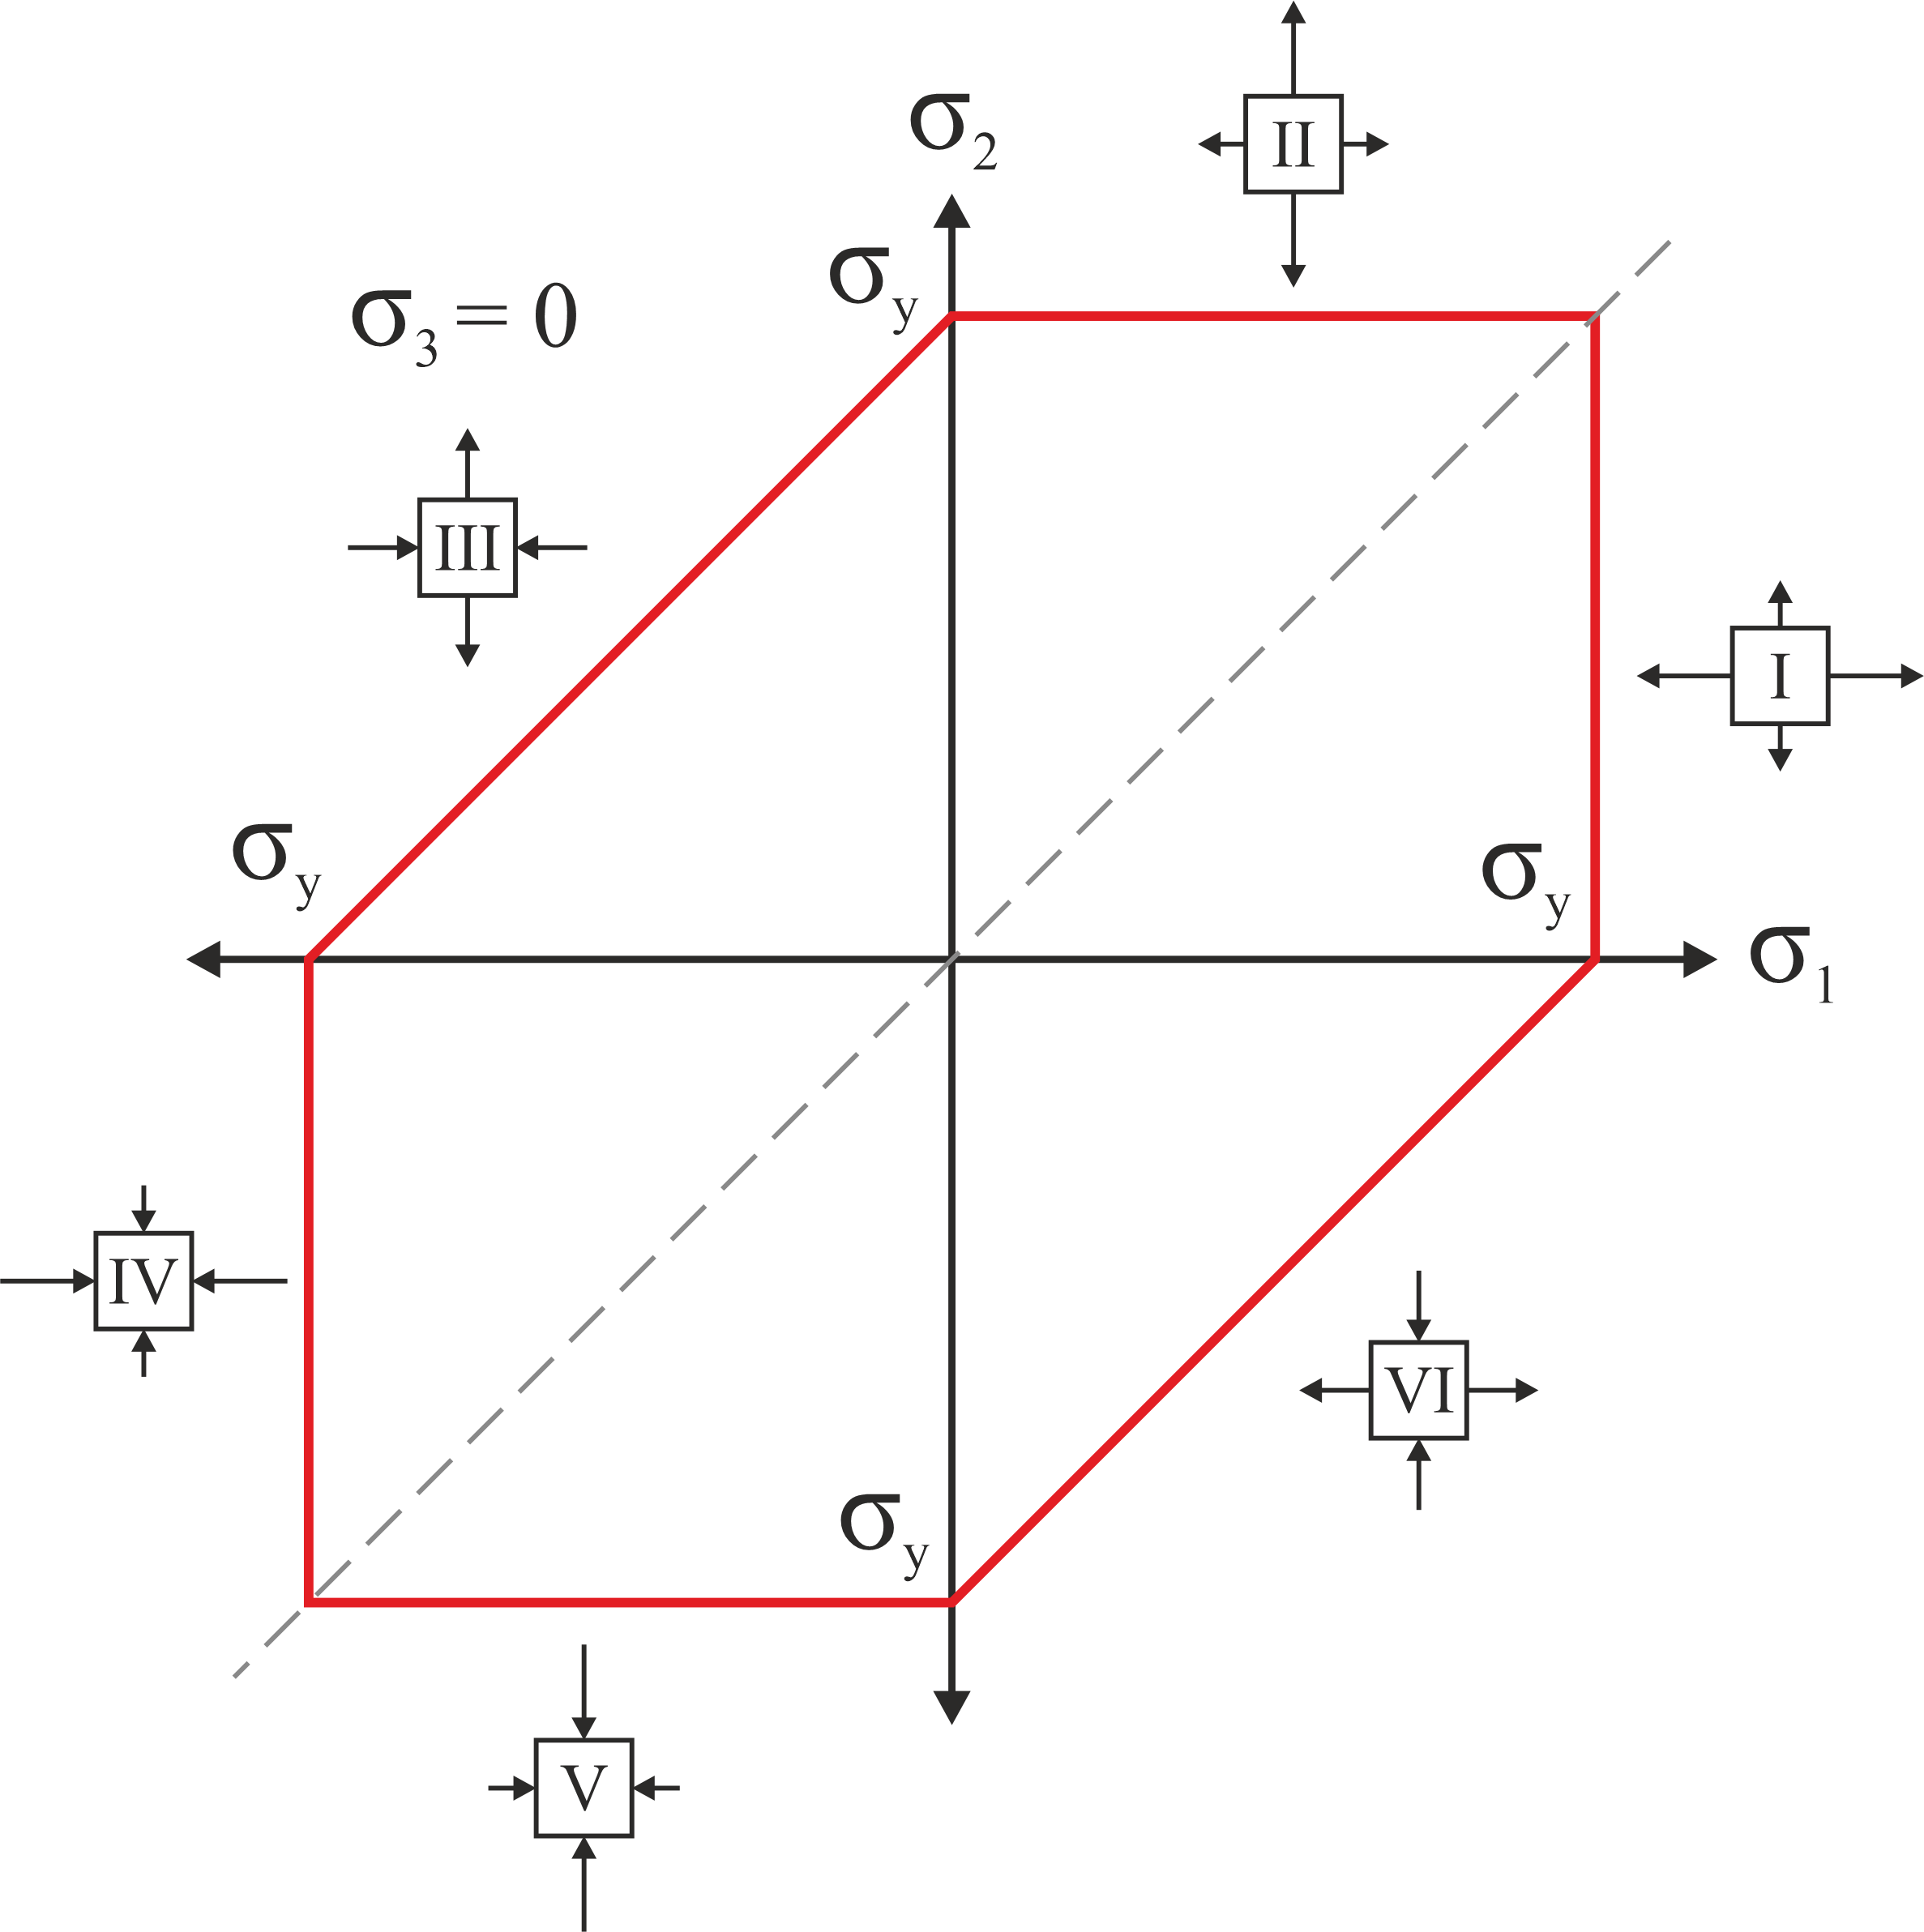
\includegraphics[width=0.4\textwidth]{images/TrescaSurface.png}
    \caption{Tresca yield surface in principal stress space. The hexagonal prism represents the yield locus, with labeled axes $\sigma_1$, $\sigma_2$, and $\sigma_3$. 
    Yielding occurs when the stress state reaches the surface. Additional description of the stress state
    are shown for every quadrants line, where the arrows indicate the direction of the stress in both axis as well
    for the magnitude \cite{hosford2005}.}
    \label{fig:tresca_surface}
\end{figure}

\begin{itemize}
    \item I: ($\sigma_1 > \sigma_2 > \sigma_3 = 0$), where $\sigma_{I} = \sigma_1$, $\sigma_{II} = \sigma_2$, and $\sigma_{III} = 0$; Therefore, $\sigma_1 = \sigma_y$
    \item II: ($\sigma_2 > \sigma_1 > \sigma_3 = 0$), where $\sigma_{I} = \sigma_2$, $\sigma_{II} = \sigma_1$, and $\sigma_{III} = 0$; Therefore, $\sigma_2 = \sigma_y$
    \item III: ($\sigma_2 > \sigma_3 = 0 > \sigma_1$), where $\sigma_{I} = \sigma_2$, $\sigma_{II} = 0$, and $\sigma_{III} = \sigma_1$; Therefore, $\sigma_2 - \sigma_1 = \sigma_y$
    \item IV: ($\sigma_3 = 0 > \sigma_2 > \sigma_1$), where $\sigma_{I} = 0$, $\sigma_{II} = \sigma_2$, and $\sigma_{III} = \sigma_1$; Therefore, $-\sigma_1 = \sigma_y$
    \item V: ($\sigma_3 = 0 > \sigma_1 > \sigma_2$), where $\sigma_{I} = 0$, $\sigma_{II} = \sigma_1$, and $\sigma_{III} = \sigma_2$; Therefore, $-\sigma_2 = \sigma_y$
    \item VI: ($\sigma_1 > \sigma_3 = 0 > \sigma_2$), where $\sigma_{I} = \sigma_1$, $\sigma_{II} = 0$, and $\sigma_{III} = \sigma_2$; Therefore, $\sigma_1 - \sigma_2 = \sigma_y$
\end{itemize}
\subsection{Von Mises yield criterion}

\hspace{2em}The von Mises yield criterion, also known as the maximum distortion energy criterion, is based on the idea
that yielding occurs when the distortion energy in the material reaches a critical value. This criterion is 
more complex compare to Tresca, as it considers the overall state of stress in the material rather than just
the maximum shear stress. The von Mises yield criterion can be expressed as follows:

\begin{equation}
    f(\boldsymbol{\sigma}) = \sigma_{eq} - \sigma_y \leq 0
\end{equation}

Where $\sigma_{eq}$ is the equivalent stress, which can be calculated using the second invariant of the deviatoric stress tensor $J_2$ as discussed in the third part.
The yield surface for the von Mises criterion can be visualized as a cylinder in the principal stress space, 
where the yield surface is defined by the condition that the equivalent stress reaches the yield stress 
$\sigma_y$. The visualization of the curve and criterion is shown as in figure~\ref{fig:vonmises_surface}.

\begin{figure}[H]
    \centering
    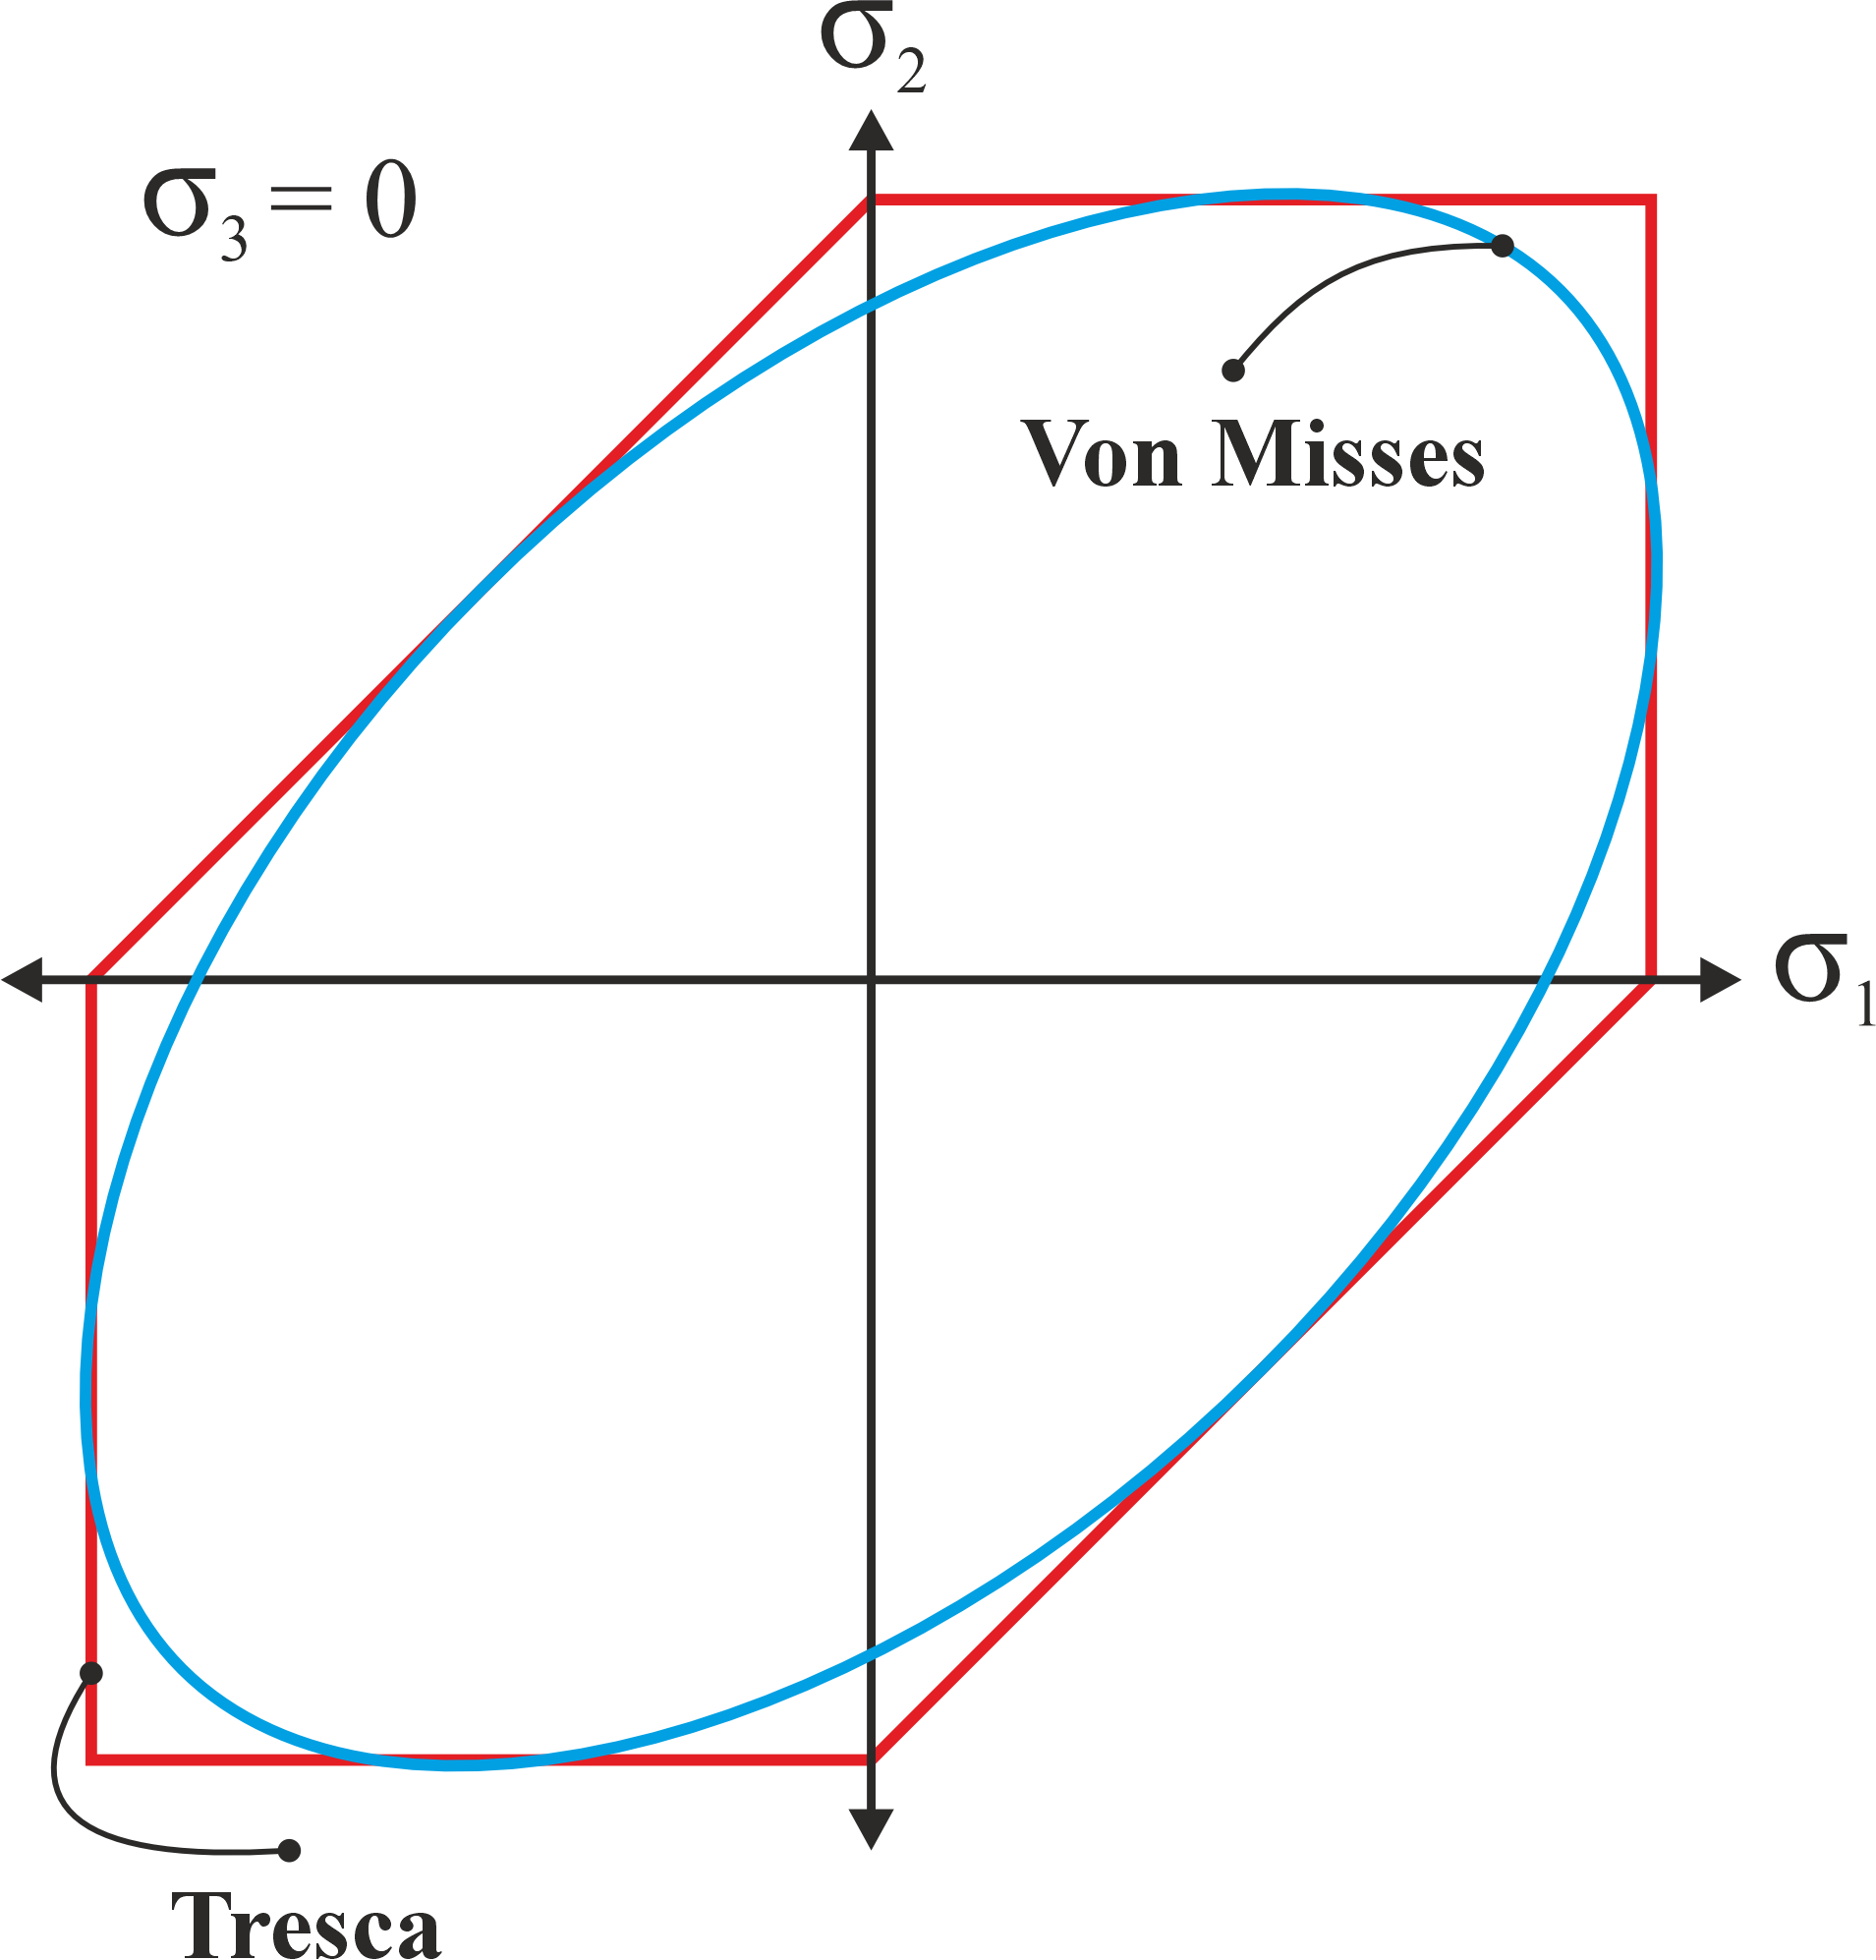
\includegraphics[width=0.35\textwidth]{images/VonMises.png}
    \caption{Von Mises yield surface in principal stress space compare to Tresca criterion. 
    The cylindrical surface represents the yield locus, with axes $\sigma_1$, $\sigma_2$, and $\sigma_3$. 
    Yielding occurs when the stress state reaches the surface. 
    The von Mises criterion provides a smooth and continuous yield surface, suitable for ductile metals.\cite{hosford2005}}
    \label{fig:vonmises_surface}
\end{figure}


\section{Evolution of yield locus with plastic strain}

\hspace{2em}A loading case scenario is not always in a monotonic condition, 
rather it can be also cyclic loading conditions. In this case,
the material will experience a repetitive loading-unloading process, which evolutions of the yield locus might occur. This process can also 
known as hardening or softening behavior (depends on the material characteristics prior to the loading). Hence, as the material
experience a plastic deformation, the yield surface will evolve with a present of the plastic strain. This 
evolution can be described in two ways, which are isotropic and kinematic hardening. 

%%Additionally, a combination of 
%%both effects can also happen in a material, which is called combined hardening.

\subsection{Isotropic hardening}

\hspace{2em}Isotropic hardening is a phenomenon as the material experience a plastic deformation,
the yield surface will expand uniformly in all directions in the stress space. This means that the material's
yield strength will increase equally for all stress states, without any change in the shape or position
of the yield surface. This type of hardening is often observed in materials that exhibit uniform
strengthening behavior, where it can be described mathematically as follows:

\begin{equation}
    \boldsymbol{\sigma}^0 = r(p) + Q_\infty(1 - e^{-bp})
\end{equation}

Where $\boldsymbol{\sigma}^0$ is the updated yield stress, $r(p)$ is the initial yield stress, 
$Q_\infty$ is the maximum increase in yield stress due to hardening, $b$ is a material constant that controls the rate of hardening, 
and $p$ is the accumulated plastic strain \cite{mehani2024modified}. The evolution of the yield surface can be visualized as follows:
\begin{figure}[H]
    \centering
    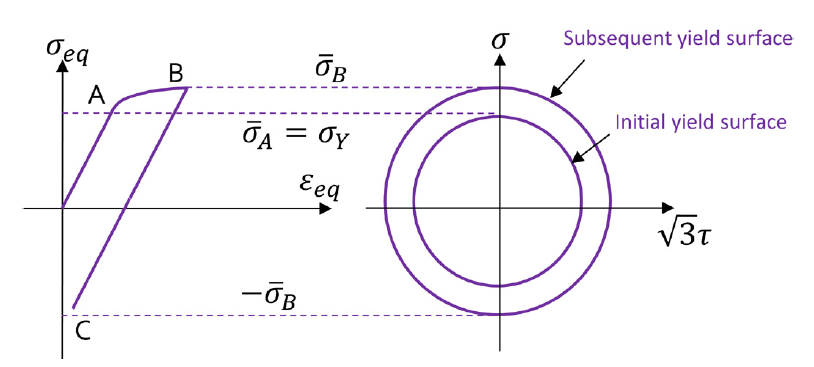
\includegraphics[width=0.6\textwidth]{images/Isotropic_Hardening.png}
    \caption{Isotropic hardening yield surface evolution in principal stress space. 
    The yield surface expands uniformly in all directions as plastic deformation occurs from the 
    value of yield stress or $\sigma_{A}$ to
    $\sigma_{B}$, 
    indicating an increase in yield strength without a change in shape or position. \cite{jahed2021cyclic}}
    \label{fig:isotropic_hardening}
\end{figure}


\subsection{Kinematic hardening}
\begin{figure}[H]
    \centering
    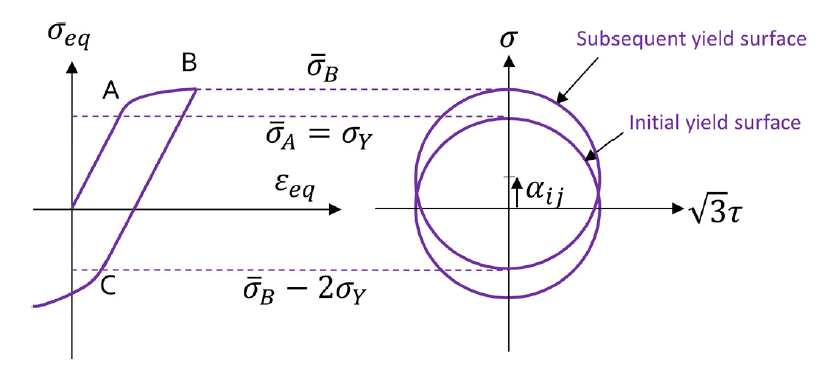
\includegraphics[width=0.6\textwidth]{images/Kinematic_Hardening.png}
    \caption{Kinematic hardening yield surface evolution in principal stress space. 
    The yield surface translates in the stress space as plastic deformation occurs from the 
    value of yield stress or $\sigma_{A}$ to
    $\sigma_{B}$, 
    indicating a shift in position without a change in size or shape. This state retains the
    value of $\sigma_y$. \cite{jahed2021cyclic}}
    \label{fig:kinematic_hardening}
\end{figure}
\hspace{2em}Different from isotropic hardening, kinematic hardening is a type of plastic hardening
where the yield surface translates in the stress space without changing its size or shape. This means that
the material's yield strength remains constant, but the position of the yield surface shifts in response
to the applied stress. This type of hardening is often observed in materials that exhibit
Bauschinger effect, where the material's response to loading and unloading is different. The mathematical
description of kinematic hardening can be expressed using the Prager's rule:

\begin{equation}
    d \alpha_{i} = \frac{2}{3}C d \boldsymbol{\varepsilon}^{p} - \gamma_{i} \alpha_{i} dp
\end{equation}

Where $\boldsymbol{\alpha}_{i}$ is the back stress tensor, $C$ is a material constant that controls 
the rate of hardening linearly, which can be determined from the von Mises yield criterion, and $d \boldsymbol{\varepsilon}_{ij}^{p}$ 
is the increment of plastic strain \cite{jahed2021cyclic}, $\gamma_{i}$ is the hardening modulus, 
and $p$ is the accumulated plastic strain. The evolution of the yield surface can be visualized
as following cited picture:


% \subsection{Combined hardening}
% \begin{figure}[H]
%     \centering
%     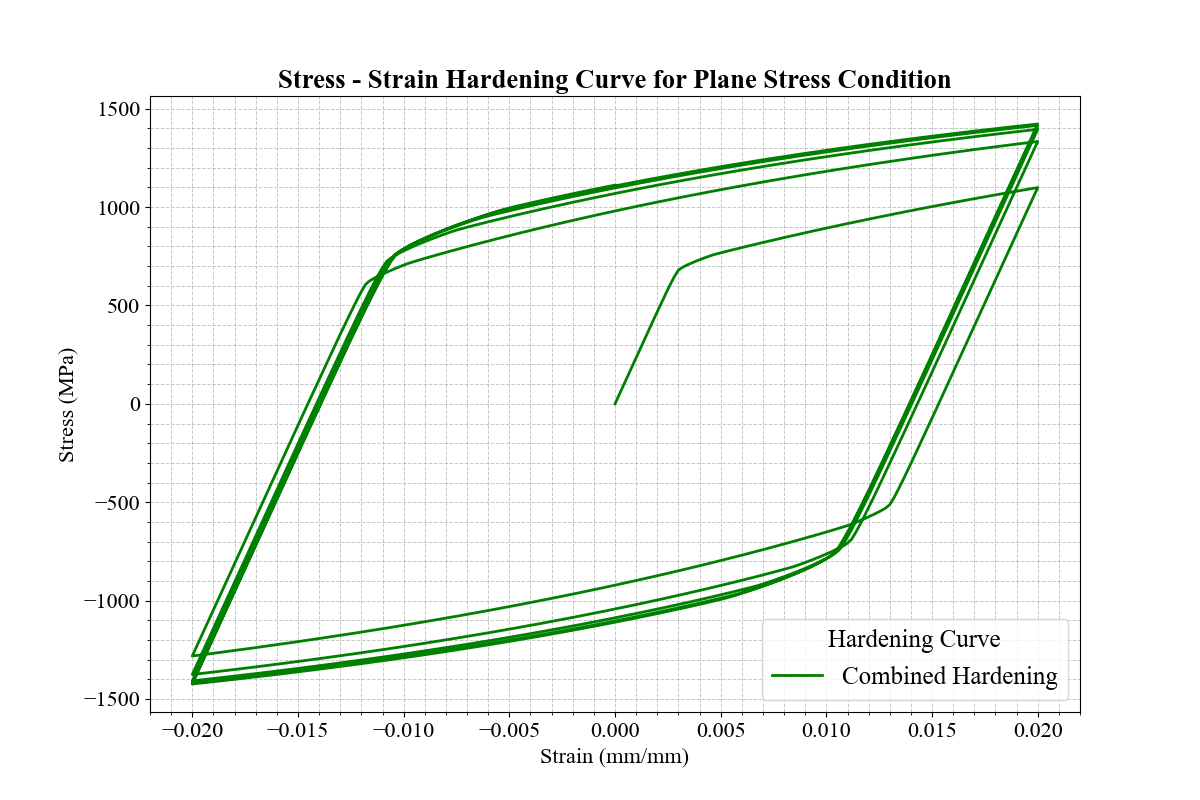
\includegraphics[width=0.6\textwidth]{images/Com_Hard.png}
%     \caption{Combined hardening yield surface evolution based on the results of assignment 2. Here it shows an 
%     expansion of the yield stress value as the cycle increases, as well as shifting of the hysteresis curve. This two
%     phenomenons indicate that the material experience a combined hardening behavior.}
%     \label{fig:combined_hardening}
% \end{figure}
%
% \hspace{2em}This type of hardening basically is the combination of both isotropic and kinematic. The model itself
% is the most realistic approach to describe material hardening behavior, since in a real case scenario
% are quite rare to find a material that only exhibit isotropic or kinematic hardening. The yield surface
% will both expand and translate in the stress space as the material experience a plastic deformation. An example of combined hardening
% is shown from assignment 2, where a plate with a hole is subjected to a cyclic loading, which combined hardening parameters
% were implemented in the material model. Hence, the results of the cyclic loading can be shown as follows:


\section{Associated flow rule}
\hspace{2em}As the material experience deformation, the stress and strain increments
follow Hooke's law at the elastic region, 
where the stress and strain relation is linear. 
However, as the material reach the yield point and experience a plastic deformation, the stress-strain
relation will be non-linear. Therefore, the stress-strain increment has reached outside the yield surface
region. To bring back the stress increment to the yield surface, a plastic flow rule is needed. This is done
to ensure that the stress state remains on the yield surface during plastic deformation. 

\hspace{2em}The plastic flow rule
is typically expressed in terms of the plastic strain rate and the yield surface. It provides a relationship
between the stress and plastic strain increments, allowing for the accurate prediction of
material behavior during plastic deformation. To ensure that the stress increment remains on the yield surface,
the plastic strain increment can be defined as follows:
\begin{equation}
    d \boldsymbol{\varepsilon}^{pl} = d \lambda \frac{\partial f}{\partial \boldsymbol{\sigma}}
\end{equation}

Where hence, the $\frac{\partial f}{\partial \boldsymbol{\sigma}}$ is the gradient of the yield surface with respect to the stress tensor, which 
is basically a normal vector to the yield surface at the current stress state, and $d \lambda$ is a 
scalar multiplier that determines the magnitude of the plastic strain increment. 
This equation states that the plastic strain increment is proportional to the normal 
vector of the yield surface, which means that the plastic deformation occurs in a direction that is 
perpendicular to the yield surface. This is known as the associated flow rule, 
which is commonly used in plasticity theory to describe the relationship between stress 
and plastic strain increments. The scalar multiplier $d \lambda$ can be obtained through the
stress rate equation and applying the consistency condition:
\begin{equation}
    d \boldsymbol{\sigma} = \boldsymbol{C} : (d \boldsymbol{\varepsilon} - d \boldsymbol{\varepsilon}^{pl}) = \boldsymbol{C} : (d \boldsymbol{\varepsilon} - d \lambda \frac{\partial f}{\partial \boldsymbol{\sigma}})
\end{equation}

The consistency condition is defined as:
\begin{equation}
    df = \frac{\partial f}{\partial \boldsymbol{\sigma}} : d \boldsymbol{\sigma} = 0
\end{equation}

By inserting the stress rate equation into the consistency condition and simplifying $\frac{\partial f}{\partial \boldsymbol{\sigma}} = n$, we can obtain an expression for the scalar multiplier $d \lambda$.
\begin{equation}
    d \lambda = \frac{n : \boldsymbol{C} : d \boldsymbol{\varepsilon}}{n : \boldsymbol{C} : n}
\end{equation}

Hence, the plastic strain increment $d \boldsymbol{\varepsilon}^{pl}$ will be used to update the constitutive 
model in the plastic region, especially to update the stress state back to the yield surface. Because in the implementation
update the stress state if the yield condition $f \geq 0$ is met. Therefore, the plastic corrector should be used to update
the stress state, which can be defined as follows:
\begin{equation}
    \boldsymbol{\sigma}_{i+1} = \boldsymbol{\sigma}_{i} + \boldsymbol{C} : (d \boldsymbol{\varepsilon} - d \boldsymbol{\varepsilon}^{pl})
\end{equation}

Where here, the $\boldsymbol{\sigma}_{i+1}$ is the updated stress state by the associated flow rule plastic increment for the plastic 
corrector case.

\section*{Crystal Plasticity}
\section{Orowan law}
\hspace{2em}After the discussion is about the mechanism of deformation of a material in a continuum and macroscopic scale,
the next discussion will be about the microscopic mechanism of plasticity, which is crystal plasticity. Hence, the first 
concept that will be discussed is the Orowan law. This law describes the basic mechanism of plastic deformation
as it describes the flow of the crystalline material dislocation movement. To describe it intuitively, 
the Orowan equation can be expressed as follows:

\begin{equation}
    \dot{\gamma} = \rho_m b v
\end{equation}

\hspace{2em}Where $\dot{\gamma}$ is the shear strain rate, $\rho_m$ is the mobile dislocation density (number
of dislocations per unit area), 
$b$ is the magnitude of the Burgers vector (measured distortion of the lattice which trigger by dislocation), 
and $v$ is the average dislocation velocity. 
This equation states that the shear strain rate is proportional to the 
product of the mobile dislocation density, the Burgers vector, and the dislocation velocity. To connect this equation
to a more phenomenological sense, the explanation can be described as following stages:
\begin{enumerate}
    \item \textbf{Microscopic Mechanism}: As a material undergoes plastic deformation, microscopically there 
    exist dislocation movements in the crystal lattice. These movements are then recorded for every slip system.
    \item \textbf{Constitutive Model for every slip system}: Each slip system has its own constitutive model, 
    which describes the relationship between the shear stress and shear strain rate. Therefore, the Orowan equation can be written
    for each slip system $\alpha$ as follows:
    \begin{equation}
        \dot{\gamma}^{(\alpha)} = \rho_m^{(\alpha)} b v^{(\alpha)}
    \end{equation}
    \item \textbf{Linking Stress and Strain Rate}: To obtain velocity $v^{(\alpha)}$, 
    the resolved shear stress $\tau^{(\alpha)}$ on the specific slip system and obstacles that hinder
    dislocation motion should be considered. 
    \item \textbf{Hardening and Microstructure Evolution}: As the material deforms plastically, the material's
    dislocation density $\rho_m^{(\alpha)}$ will evolve due to the change of the microstructure, which then will harden and resist for 
    further dislocation motion. This evolution can be described by a hardening law, which relates
    the change in dislocation density to the plastic strain rate.
\end{enumerate}

\section{Resolved shear stress}
\begin{figure}[H]
    \centering
    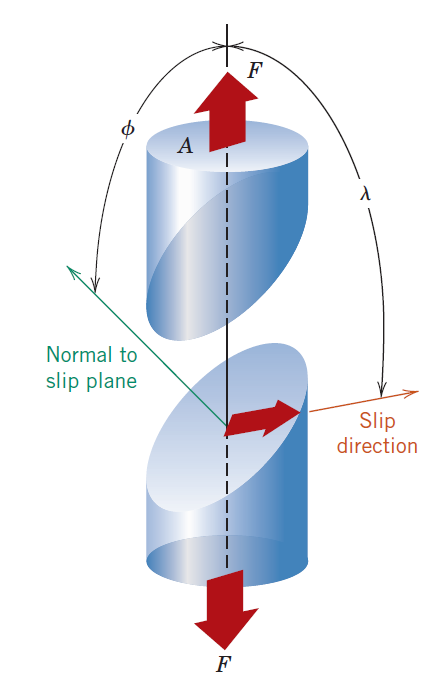
\includegraphics[width=0.25\textwidth]{images/RSS_New.png}
    \caption{Visualization of resolved shear stress on a single crystal under an applied uniaxial stress $\sigma$. 
    The slip plane is defined by the normal vector $n$, and the slip direction is defined by the vector $s$. 
    The angle between the applied stress direction and the slip plane normal is $\phi$, and the angle between 
    the applied stress direction and the slip direction is $\lambda$. \cite{callister2010}}
    \label{fig:resolved_shear_stress}
\end{figure}

\hspace{2em}In a crystallographic scale of material, there exist a slip system, which is a combination
of the movement along the slip plane and slip direction. The slip plane is defined as the plane by which 
the dislocation motion occurs in a crystal lattice, while the slip direction is the movement direction 
of the dislocation within the slip plane. Therefore, the movement will occur in the slip system as a driving
force is applied to the material, which called resolved shear stress. This stress is calculated based
on the applied tensor as well as the orientation of the slip system and the normal vector prior to the slip plane.
The resolved shear stress $\tau$ on a specific slip system can be calculated using the following equation:

\begin{equation}
    \tau = \boldsymbol{s} : \boldsymbol{\sigma} : \boldsymbol{n}
\end{equation}

Where $\boldsymbol{s}$ is the slip direction unit vector, $\boldsymbol{n}$ is the 
slip plane normal unit vector, and $\boldsymbol{\sigma}$ is the applied stress tensor. 
The colon operator (:) denotes the double contraction of tensors for tensor notation. Hence, the resolved shesr stress
can be used to calculate the velocity of dislocation movement in the Orowan equation, which is denote as following 
relation:

\begin{equation}
    v = \frac{\tau b}{B}
\end{equation}

Where b is the magnitude of the Burgers vector and B is the drag coefficient that is material and temperature
dependent. 


\section{Finite strain formulation}
\hspace{2em}In a crystal plasticity model, the deformation of a material is often in large strain,
which means that the deformation is not small enough to be approximated by linear plasticity. Therefore, a finite strain
formulation is needed to model such huge deformation. To obtain such flow rule using the large deformation framework, a step-by-step
approach can be done as follows:
\begin{enumerate}
    \item \textbf{Deformation Gradient}: The deformation gradient $\boldsymbol{F}$ is defined as the mapping
    from the reference to the current configuration. Hence, it can be expressed as follows:
    \begin{equation}
        \boldsymbol{F} = \frac{\partial \boldsymbol{x}}{\partial \boldsymbol{X}}
    \end{equation}
    Where $\boldsymbol{x}$ is the current position vector and $\boldsymbol{X}$ is the reference position vector.
    \item \textbf{Multiplicative Decomposition}: The deformation gradient can be decomposed into elastic and 
    plastic parts, which is known as the multiplicative decomposition:
    \begin{equation}
        \boldsymbol{F} = \boldsymbol{F}^{e} \boldsymbol{F}^{p}
    \end{equation}
    Where $\boldsymbol{F}^{e}$ is the elastic deformation gradient and $\boldsymbol{F}^{p}$ is the plastic 
    deformation gradient. In ths finite strain framework, the plastic deformation gradient
    $\boldsymbol{F}^{p}$ describes the irreversible deformation due to dislocation motion, while the elastic
    deformation gradient $\boldsymbol{F}^{e}$ describes the reversible deformation due to elastic stretching
    and rotation of the crystal lattice. The plastic part will then be used to describe the crystal plasticity
    flow rule. 

    \item \textbf{Plastic Velocity Gradient}: The plastic velocity gradient $\boldsymbol{L}^{p}$ can be 
    defined as follows:
    \begin{equation}
        \boldsymbol{L}^{p} = \dot{\boldsymbol{F}}^{p} (\boldsymbol{F}^{p})^{-1}
    \end{equation}

    Where $\dot{\boldsymbol{F}}^{p}$ is the time derivative of the plastic deformation gradient. Hence, the velocity
    gradient will be used to describe the crystal plasticity flow rule, which then can be expressed as follows:
    
    \begin{equation}
        \boldsymbol{L}^{p} = \sum_{\alpha} \dot{\gamma}^{(\alpha)} \boldsymbol{s}^{(\alpha)} \otimes \boldsymbol{n}^{(\alpha)} 
\end{equation}
    Where $\dot{\gamma}^{(\alpha)}$ is the shear strain rate on slip system $\alpha$, $\boldsymbol{s}^{(\alpha)}$ is the slip direction unit vector,
    $\boldsymbol{n}^{(\alpha)}$ is the slip plane normal unit vector, and $\otimes$ denotes the tensor product. This velocity gradient 
    will be used as the basis to calculate the plastic deformation gradient by relating it with the crystallographic slip system. 
\end{enumerate}

\section{Crystal plasticity flow rule}
\hspace{2em}After all the ingredients and relations are obtained, now rise the question on how to implement the flow rule in crystal plasticity
scale. Because in a crystal plasticity model, anisotropic behavior is considered due to the facts that the crystallographic structure
are having a specific orientation for each of them. Therefore, capturing the history-dependent parameters is important in order to
model such behavior. The flow rule or the slip rate law can be expressed as follows:
\begin{equation}
    \dot{\gamma}^{(\alpha)} = \dot{\gamma}_0 \left( \frac{|\tau^{(\alpha)}|}{\tau^{(\alpha)}_{c}} \right)^{n} \text{sign}(\tau^{(\alpha)})
\end{equation}

\hspace{2em}Where $\dot{\gamma}^{(\alpha)}$ is the shear strain rate on slip system $\alpha$, $\dot{\gamma}_0$ is a reference shear 
strain rate, $\tau^{(\alpha)}$ is the resolved shear stress on slip system $\alpha$, $\tau^{(\alpha)}_{c}$ is the 
critical resolved shear stress (CRSS) for slip system $\alpha$, and $n$ is a rate sensitivity exponent that controls the
sensitivity of the slip rate to the resolved shear stress. The sign function ensures that the slip rate has the same
direction as the resolved shear stress.

\hspace{2em}To connect it to the dislocation theory, by means of Orowan law, the average dislocation velocity can be expressed using
thermally active model, which can be written as follows:
\begin{equation}
     v^{(\alpha)} \propto b \nu \exp \left( -\frac{\Delta G(\tau^{(\alpha)})}{kT} \right)
\end{equation}

\hspace{2em}To sum up the implementation of the crystal plasticity flow rule, 
the shear strain rate $\dot{\gamma}^{(\alpha)}$ on each slip system will resolve the slip rate $\dot{\gamma}^{(\alpha)}$.
This slip rate will then be used to update the plastic velocity gradient $\boldsymbol{L}^{p}$, which then
will be used to update the plastic deformation gradient $\boldsymbol{F}^{p}$. The plastic deformation gradient
will then be used to update the total deformation gradient $\boldsymbol{F}$, which then will be used to calculate
the stress state in the material. This process will be repeated for each time step in the simulation. A graphical description
of the described process is presented as follows:
\vspace{1em}
\begin{figure}[H]
    \centering
    \includegraphics[width=0.8\textwidth]{images/graphical_FlowRule.png}
    \caption{Graphical representation of the crystal plasticity flow rule process, showing the update sequence from slip rate to stress state.}
    \label{fig:graphical_flow_rule}
\end{figure}

\bibliographystyle{plain}
\bibliography{bibliography_CIBB_file.bib}
\newpage
\section*{Appendix: Large-Language Models (LLMs) use in this report based on GPT@RUB}


%% ---------------------------------------- %%



\begin{summary}{Prompt 1: Explanation of crystal plasticity flow rule}
\textbf{Prompt:} "Could you explain the crystal plasticity flow rule more structured and step-by step so that we get sort of like an input and output from this flow rule? And could you explain what outcomes that we need from the output for the numerical integration scheme?"
\vspace{1em}

\textbf{Response:}

Absolutely! Here’s a step-by-step, structured explanation of the crystal plasticity flow rule, focusing on its role as a constitutive law in a numerical (e.g., finite element) integration scheme. I’ll highlight the inputs, outputs, and the key outcomes needed for numerical integration.
\textbf{Step-by-step, structured explanation} of the crystal plasticity flow rule, focusing on its role as a constitutive law in numerical (e.g., finite element) integration.  

\section*{1. Step-by-Step Structure of the Flow Rule}

\subsection*{Step 1: Inputs}
At each time increment:
\begin{itemize}
    \item Deformation gradient: \( \mathbf{F} \)  
    \item Stress state: \( \boldsymbol{\sigma} \) or \( \boldsymbol{\tau} \)  
    \item Slip geometry: \( \mathbf{s}^\alpha, \mathbf{m}^\alpha \)  
    \item Internal variables: \( \tau_c^\alpha, \gamma^\alpha \), dislocation densities  
    \item Material parameters: \( \dot{\gamma}_0, n, h^{\alpha\beta}, b \), etc.  
\end{itemize}

\subsection*{Step 2: Resolved Shear Stress}
\[
\tau^\alpha = \mathbf{S}^\alpha : \boldsymbol{\tau}, 
\qquad \mathbf{S}^\alpha = \mathbf{s}^\alpha \otimes \mathbf{m}^\alpha
\]

\subsection*{Step 3: Flow Rule (Slip Rate Law)}
\[
\dot{\gamma}^\alpha = \dot{\gamma}_0 \left| \frac{\tau^\alpha}{\tau_c^\alpha} \right|^n \operatorname{sign}(\tau^\alpha)
\]
\end{summary}
\newpage
%% ---------------------------------------- %%

\begin{summary}{Prompt 1: Explanation of crystal plasticity flow rule}
Rate-independent case:
\[
\dot{\gamma}^\alpha \neq 0 \quad \text{iff} \quad |\tau^\alpha| = \tau_c^\alpha
\]



\subsection*{Step 4: Plastic Velocity Gradient}
\[
\mathbf{L}^p = \sum_\alpha \dot{\gamma}^\alpha \mathbf{S}^\alpha
\]

\subsection*{Step 5: Plastic Deformation Gradient}
\[
\mathbf{F}^p_{n+1} = \exp(\mathbf{L}^p \Delta t)\mathbf{F}^p_n
\]
or, small increments:
\[
\mathbf{F}^p_{n+1} \approx (\mathbf{I} + \mathbf{L}^p \Delta t)\mathbf{F}^p_n
\]

\subsection*{Step 6: Update Internal Variables (Hardening Law)}
\[
\tau_{c_{n+1}}^\alpha = \tau_c^{\alpha_n} + \sum_\beta h^{\alpha\beta} |\Delta \gamma^\beta|,
\qquad \Delta \gamma^\beta = \dot{\gamma}^\beta \Delta t
\]

\section*{2. Summary Table: Inputs and Outputs}
\begin{tabular}{|c|c|c|}
\hline
\textbf{Step} & \textbf{Input} & \textbf{Output} \\
\hline
1 & \( \mathbf{F}, \boldsymbol{\tau}, \mathbf{s}^\alpha, \mathbf{m}^\alpha, \tau_c^\alpha, \gamma^\alpha \) & -- \\
2 & \( \boldsymbol{\tau}, \mathbf{s}^\alpha, \mathbf{m}^\alpha \) & \( \tau^\alpha \) \\
3 & \( \tau^\alpha, \tau_c^\alpha, \dot{\gamma}_0, n \) & \( \dot{\gamma}^\alpha \) \\
4 & \( \dot{\gamma}^\alpha, \mathbf{s}^\alpha, \mathbf{m}^\alpha \) & \( \mathbf{L}^p \) \\
5 & \( \mathbf{L}^p, \mathbf{F}^p_n \) & \( \mathbf{F}^p_{n+1} \) \\
6 & \( \dot{\gamma}^\alpha, \tau_c^\alpha \) & \( \tau_{c_{n+1}}^{\alpha} \) \\
\hline
\end{tabular}


\section*{3. Key Outcomes for Integration}
\begin{enumerate}
    \item Updated plastic deformation gradient \( \mathbf{F}^p_{n+1} \)  
    \item Updated internal variables \( \tau_{c_{n+1}}^\alpha, \gamma^\alpha_{n+1} \)  
    \item Consistent tangent moduli (for implicit schemes)  
\end{enumerate}
\end{summary}


%% ---------------------------------------- %%

\begin{summary}{Prompt 1: Explanation of crystal plasticity flow rule}
\section*{4. Flowchart (Conceptual)}
\begin{tabular}{l}
\textbf{Input:} $\mathbf{F}$, $\boldsymbol{\tau}$, $\mathbf{s}^\alpha$, $\mathbf{m}^\alpha$, $\tau_c^\alpha$, $\gamma^\alpha$ \\
\quad $\downarrow$ \\
Compute $\tau^\alpha = \mathbf{S}^\alpha : \boldsymbol{\tau}$ \\
\quad $\downarrow$ \\
Evaluate flow rule: $\dot{\gamma}^\alpha = \dot{\gamma}_0 \left| \frac{\tau^\alpha}{\tau_c^\alpha} \right|^n \operatorname{sign}(\tau^\alpha)$ \\
\quad $\downarrow$ \\
Compute $\mathbf{L}^p = \sum_\alpha \dot{\gamma}^\alpha \mathbf{S}^\alpha$ \\
\quad $\downarrow$ \\
Update $\mathbf{F}^p$ \\
\quad $\downarrow$ \\
Update $\tau_c^\alpha$, $\gamma^\alpha$ (hardening) \\
\quad $\downarrow$ \\
\textbf{Output:} $\mathbf{F}^p_{n+1}$, $\tau_{c_{n+1}}^\alpha$, $\gamma_{n+1}^\alpha$ \\
\end{tabular}
\vspace{1em}
\section*{5. In Summary}
\begin{itemize}
    \item \textbf{Input:} deformation, stress, slip geometry, internal variables  
    \item \textbf{Flow rule:} slip rates from resolved shear stress and slip resistance  
    \item \textbf{Output:} updated \( \mathbf{F}^p \), internal variables  
    \item \textbf{Use:} update stress, evolve history, provide tangents  
\end{itemize}
\end{summary}


%% ---------------------------------------- %%

\begin{summary}{Prompt 2: Explanation of Finite Strain Formulation}
\textbf{Prompt:} "What is finite strain formulation in Crystal Plasticity?"
\vspace{1em}

\textbf{Response:}

\vspace{1em}

\textbf{Finite strain formulation in crystal plasticity} refers to the mathematical
and computational framework used to model the deformation of crystalline
materials (such as metals) when they undergo large, or finite, deformations.
This is particularly important for accurately capturing the behavior of
materials where the deformation is not small, and the crystal lattice undergoes
significant rotations and stretches.
\end{summary}

\begin{summary}{Prompt 2: Explanation of Finite Strain Formulation}
\subsection*{Key Concepts}

\paragraph{1. Crystal Plasticity}
Crystal plasticity is a theory that describes how crystals (grains) in a
polycrystalline material deform, primarily by slip along specific
crystallographic planes and directions (slip systems). It accounts for the
anisotropic (direction-dependent) nature of crystal deformation.

\paragraph{2. Finite Strain Kinematics}
In the finite strain regime, the total deformation is large, so linear
approximations are not valid. The deformation gradient tensor $\mathbf{F}$ is
used to describe the transformation from the reference (undeformed) to the
current (deformed) configuration.

\paragraph{3. Multiplicative Decomposition}
A central idea in finite strain crystal plasticity is the multiplicative
decomposition of the deformation gradient:
\begin{equation}
    \mathbf{F} = \mathbf{F}^e \mathbf{F}^p,
\end{equation}
where
\begin{itemize}
  \item $\mathbf{F}^e$: Elastic part (lattice stretching and rotation),
  \item $\mathbf{F}^p$: Plastic part (slip and twinning on crystallographic planes).
\end{itemize}
This decomposition separates the reversible (elastic) and irreversible (plastic)
parts of the deformation, which is crucial for modeling crystal behavior at
large strains.

\paragraph{4. Slip Systems and Plastic Flow}
Plastic deformation is modeled as the sum of shearing on multiple slip systems:
\begin{equation}
    \dot{\mathbf{F}}^p (\mathbf{F}^p)^{-1}
    = \sum_{\alpha} \dot{\gamma}^{\alpha}\,
      \mathbf{s}^{\alpha} \otimes \mathbf{m}^{\alpha},
\end{equation}
where
\begin{itemize}
  \item $\dot{\gamma}^{\alpha}$: Shear rate on slip system $\alpha$,
  \item $\mathbf{s}^{\alpha}$: Slip direction,
  \item $\mathbf{m}^{\alpha}$: Slip plane normal.
\end{itemize}

\paragraph{5. Stress and Constitutive Laws}
Stress measures compatible with finite strains (e.g., Kirchhoff or Cauchy
stress) are used. Constitutive laws relate the resolved shear stress on each
slip system to the slip rate, often using flow rules and hardening laws.

\paragraph{6. Numerical Implementation}
Finite strain crystal plasticity is often implemented in finite element codes
to simulate the behavior of polycrystalline aggregates under large
deformations, such as in metal forming, texture evolution, and failure
analysis.
\end{summary}

\begin{summary}{Prompt 2: Explanation of Finite Strain Formulation}
\subsection*{Summary Table}

\begin{center}
\begin{tabular}{@{}lll@{}}
\toprule
Aspect & Small Strain C.Plasticity & Finite Strain C.Plasticity \\
\midrule
Deformation    & Linear (small)            & Nonlinear (large) \\
Kinematics     & Additive decomposition    & Multiplicative decomposition \\
Strain Measures& Linear strain tensor      & Deformation gradient, Green--Lagrange \\
Stress Measures& Cauchy stress             & Cauchy, Kirchhoff, or Piola--Kirchhoff \\
Applications   & Low-strain problems       & Large deformations, texture evolution \\
\bottomrule
\end{tabular}
\end{center}

\subsection*{In Summary}
\noindent
\textbf{Finite strain formulation in crystal plasticity} is a nonlinear,
physically based approach that models the large deformation behavior of crystals
by decomposing the total deformation into elastic and plastic parts, tracking
slip on crystallographic planes, and using appropriate stress and strain
measures. This allows for accurate simulation of the mechanical response and
microstructural evolution of crystalline materials under large strains.
\end{summary}

\begin{summary}{Prompt 3: Explanation of Orowan's Law}
\textbf{Prompt:} "Could you explain the orowan's law in crystal plasticity in more phenomenologically case?"
\vspace{1em}

\textbf{Response:}

\subsection*{What We Observe}
When you deform a metal (for example, by bending a paperclip), you notice that:
\begin{itemize}
  \item At first, it bends easily (elastic deformation).
  \item If you bend it further, it stays bent (plastic deformation).
  \item The more you bend it, the harder it gets to bend further (work hardening).
\end{itemize}

\subsection*{What’s Happening Inside?}
\begin{itemize}
  \item Plastic deformation in metals is not due to the breaking of atomic bonds
  all at once, but rather due to the movement of dislocations---tiny line
  defects in the crystal structure.
  \item As you deform the metal, these dislocations move, multiply, and interact.
\end{itemize}
\end{summary}

\begin{summary}{Prompt 3: Explanation of Orowan's Law}
\subsection*{Orowan’s Law Connects the Dots}
Orowan’s law provides a simple, observable relationship:
\[
\text{Plastic strain rate} = 
\text{(Number of moving dislocations)} \times
\text{(Distance per event)} \times
\text{(Velocity)}
\]

Mathematically:
\begin{equation}
  \dot{\varepsilon}_p = \rho_m \, b \, v ,
\end{equation}
where
\begin{itemize}
  \item $\dot{\varepsilon}_p$: Plastic strain rate (rate of permanent deformation),
  \item $\rho_m$: Density of mobile dislocations,
  \item $b$: Burgers vector magnitude (dislocation step size),
  \item $v$: Average dislocation velocity (depends on stress and temperature).
\end{itemize}

\subsection*{Phenomenological Implications}
\begin{itemize}
  \item \textbf{Work Hardening:} As deformation progresses, $\rho_m$ increases.
  More dislocations are available, but they hinder each other’s motion,
  increasing strength.
  \item \textbf{Rate Sensitivity:} Faster deformation requires higher
  dislocation velocity $v$, often demanding higher applied stress.
  \item \textbf{Temperature Effects:} At higher temperatures, dislocations move
  more easily (higher $v$), making the material softer.
\end{itemize}

\subsection*{Everyday Example}
Imagine a crowded hallway (the crystal) with people (dislocations) trying to
move from one end to the other:
\begin{itemize}
  \item With few people, motion is easy (low dislocation density).
  \item With many people, collisions make motion harder (work hardening).
  \item If everyone moves faster (higher strain rate), congestion increases,
  requiring more effort to move.
\end{itemize}
\end{summary}

\newpage
\begin{summary}{Prompt 3: Explanation of Orowan's Law}
\subsection*{Summary}
Phenomenologically, Orowan’s law tells us:
\begin{itemize}
  \item The rate of plastic deformation is directly related to the number of
  moving dislocations, their travel distance, and their velocity.
  \item It explains key behaviors such as work hardening, rate sensitivity, and
  temperature dependence in metals.
\end{itemize}

\noindent
\textbf{In essence:} Orowan’s law bridges what we observe (macroscopic metal
deformation) with the underlying mechanism (dislocation motion), providing a
simple and powerful explanation of plasticity in crystalline materials.
\end{summary}
\end{document} 

